\documentclass[10pt,a4paper]{scrartcl}
\usepackage[left=2cm,right=2cm,top=2cm,bottom=2cm]{geometry}

%Language settings
\usepackage[utf8]{inputenc}
\usepackage[T1]{fontenc}
\usepackage[german]{babel}
\usepackage[babel, german=quotes]{csquotes}

%Fonts
\usepackage{lmodern}
\usepackage{mathrsfs}

%Packages
\usepackage{amsmath}
\usepackage{amsfonts}
\usepackage{amssymb}
\usepackage{xcolor}
\usepackage{graphicx}
\usepackage{float}
\usepackage{caption}
\usepackage[linesnumbered,ruled]{algorithm2e}
\usepackage{multicol}
\usepackage{parskip}

%Biblatex
\usepackage{hyperref}
\usepackage[style=alphabetic]{biblatex}
\addbibresource{bibliography.bib}

%Title, author, etc.
\title{Support Vector Machines mit Kerneln}
\author{Jonas Krug, Hendrik Sieck und Tim Schlottmann \\ TU Hamburg}
\date{\today}

\begin{document}

    \maketitle

    \begin{multicols}{2}

        \section{Abstract}

        \section{Motivation}

        \section{Support vector machines -- Grundlagen}
        Support Vector Maschinen sind ein binärer Klassifizierer. Datenmengen werden also in zwei Klassen eingeteilt. Zur Unterteilung der Klassen wird eine Hyperebene benutzt. Wie die Unterteilung stattfindet soll in diesem Abschnitt erklärt werden.

            \subsection{Definitionen}
                Folgende Definitionen bilden die Grundlage für SVMs:

                \begin{itemize}
                    \item Anzahl an Datenpunkten: $ m \in \mathbb{R} $
                    \item Input: $ \boldsymbol{x} \in \mathbb{R}^N $
                    % \item Input $ \boldsymbol{x} := \{ \boldsymbol{x}_1, \dots, \boldsymbol{x}_m \} \text{, } \boldsymbol{x} \in \mathbb{R}^N $
                    \item Output: $ y \in \{ -1, +1 \} $
                    \item Trainingsset: $S \in (\mathbb{R}^N \times \{ -1, +1 \})^m $
                \end{itemize}

                Ziel ist es, eine Hypothese zu finden, die einen Input $\boldsymbol{x}$ auf eine der beiden Klassen $y$ abbildet: \begin{align*}
                    h: \mathbb{R}^N &\to \{ +1, -1 \} \\
                    \boldsymbol{x} &\mapsto y
                \end{align*}
            \subsection{Hyperebene}
                Betrachten wir ein Trainingsset $S$ mit eingezeichneter Hyperebene $H$ wie in Abbildung \ref{fig:hyperplanes}. Es fällt auf, dass ein Spalt (engl. margin) entsteht, dessen Grenzen sich durch zwei weitere Hilfsebenen $H_+$ und $H_-$ darstellen lassen. $H_+$ und $H_-$ sind hierbei parallel zu $H$. In Abbildung \ref{fig:hyperplanes} ist $H_+$ die Begrenzung zur $+1$-Klasse und $H_-$ die Begrenzung zur $-1$-Klasse. Die Vektoren, durch die die Hilfsebenen verlaufen, heißen Supportvektoren und sind in der Abbildung schwarz umrandet.
                \begin{figure}[H]
                    \centering{
                        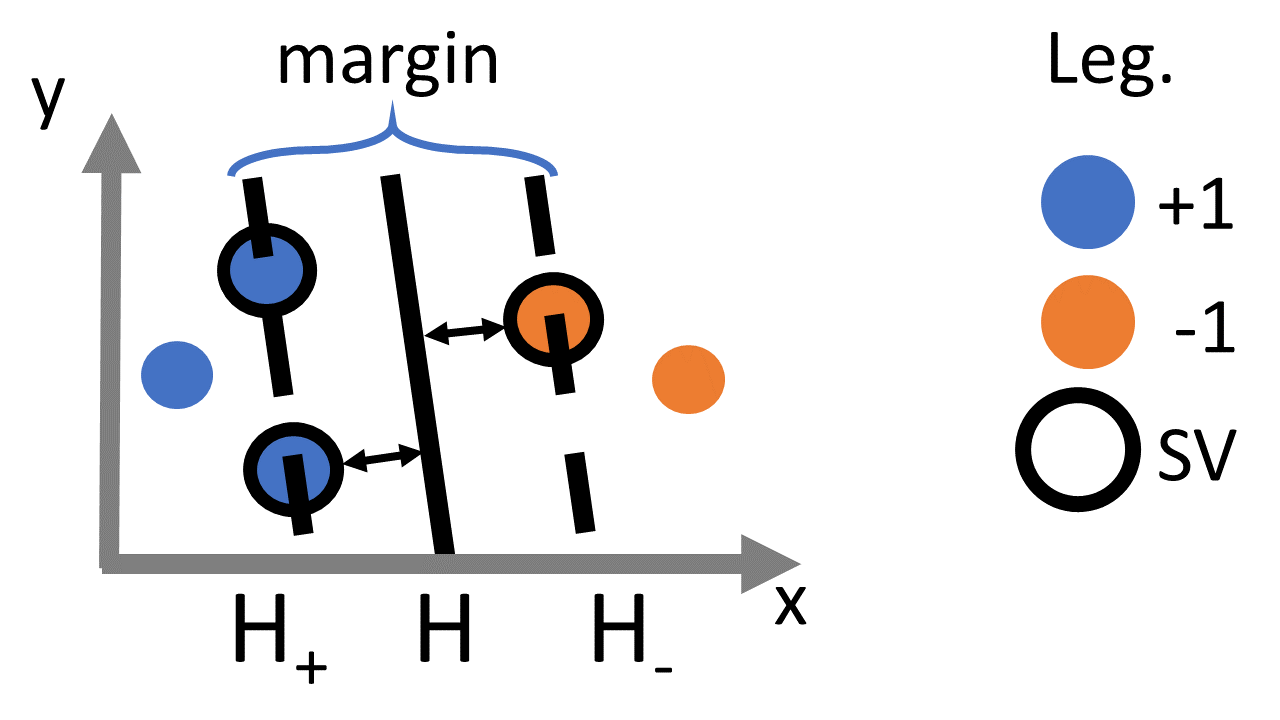
\includegraphics[width=0.66\columnwidth]{img_tim/Folie7.PNG}
                        \caption{Hyperebene $H$ zur Trennung der beiden Klassen $+1$ und $-1$}
                        \label{fig:hyperplanes}
                    }
                \end{figure}
                Nun gilt es die Hypothese zu finden. Hierfür betrachten wir zuerst die Hyperbenengleichung $H = \boldsymbol{w}^T \boldsymbol{x} + b = 0$. 
                Hierbei werden die Parameter $\boldsymbol{w}$ und $b$ so gewählt, dass für die Supportvektoren gilt: $y_i ( \boldsymbol{w}^T \boldsymbol{x}_i + b ) = 1$
                So lässt sich die Hypothese wie folgt definieren:
                \begin{equation*}
                    h(\boldsymbol{x}_i) = \begin{cases}
                        +1 & \text{ wenn } \boldsymbol{w}^T \boldsymbol{x}_i + b \geq 0 \\
                        -1 & \text{ wenn } \boldsymbol{w}^T \boldsymbol{x}_i + b \leq 0
                    \end{cases}
                \end{equation*}

            \subsection{Minimierungsproblem}
                Die algorithmische Bestimmung der Parameter $\boldsymbol{w}$ und $b$ erfolgt über ein Minimierungsproblem. Die Spalte zwischen den Hilfsebenen $H_+$ und $H_-$ soll maximiert werden. Über die Projektionseigenschaft des Skalarproduktes lässt sich die Breite der Spalte über den Ausdruck $\frac{2}{\Vert \boldsymbol{w} \Vert}$ bestimmen. Die Breite der Spalte soll nun maximiert werden, was zu folgendem Minimierungsproblem führt:
                \begin{align*}
                    & \max_{\boldsymbol{w}, b} \frac{2}{\Vert \boldsymbol{w} \Vert} \Leftrightarrow \min_{\boldsymbol{w}, b} \Vert \boldsymbol{w} \Vert \Leftrightarrow \min_{\boldsymbol{w}, b} \frac{1}{2} \Vert \boldsymbol{w} \Vert^2 \\
                    & \text{u.d.N. } y_i ( \boldsymbol{w}^T \boldsymbol{x}_i + b ) - 1 \geq 0
                \end{align*}
                Durch die Verwendung von Lagrange Multiplikatoren lässt sich das Minimierungsproblem in eine Form bringen, die nur noch von der Langrangevariable $\alpha$ sowie den Supportvektoren bzw. den neu zu klassifizierenden Vektoren abhängt:
                \begin{align*}
                    \boldsymbol{w} &= \sum_i \alpha_i y_i \boldsymbol{x}_i \\
                    \sum_i \alpha_i y_i &= 0 \\
                    h(\boldsymbol{x}) &= \begin{cases}
                        +1 & \sum_i \alpha_i y_i \boldsymbol{x}_i^T \boldsymbol{x} + b \geq 0 \\
                        -1 & \sum_i \alpha_i y_i \boldsymbol{x}_i^T \boldsymbol{x} + b \leq 0
                    \end{cases}
                \end{align*}
        \section{Kernel Trick -- Jonas}

        \section{Tipps und Tricks zu Machine Learning und SVMs}
            Sämtlicher Code, Erläuterungen und das Präsentations-Skript sind online verfügbar: \url{https://github.com/NIPE-SYSTEMS/support-vector-machine}
            
            Unten auf der Repository-Seite (siehe Link) befindet sich eine Beschreibung zu allen wichtigen Dateien im Repository.


    \end{multicols}
\end{document}